\documentclass[a4paper,12pt,oneside]{report}

\usepackage{fancyhdr}
\usepackage[magyar]{babel}
\usepackage{t1enc}
\usepackage[utf8]{inputenc}
\usepackage{graphicx}
\usepackage{todonotes}
\usepackage[section,numbib,nottoc]{tocbibind}
\usepackage{hyperref}
\usepackage{amssymb}
\usepackage{booktabs}
\usepackage{pdflscape}
\usepackage{formai_kovetelmenyek}
\usepackage{pdfpages}
\usepackage{fixltx2e}
\usepackage{tikz}
\usepackage{floatrow}

\usepackage{array} % for defining a new column type
\usepackage{varwidth} %for the varwidth minipage environment


\hypersetup{
    unicode=false,
    pdfauthor={Kránitz Gábor},
    pdftitle={Tűzfalak tesztelése hálózati forgalom visszajátszással}
}

\lstset{
     basicstyle = \ttfamily\footnotesize
    ,breaklines = true
    ,prebreak   = \raisebox{0ex}[0ex][0ex]{\ensuremath{\hookleftarrow}}
    ,extendedchars = true
    ,literate={á}{{\'a}}1 {ó}{{\'o}}1 {é}{{\'e}}1 {í}{{\'i}}1 {ő}{{\~o}}1 {ö}{{\"o}}1 {ű}{{\'u}}1
}

\hyphenation{Google}

\title{Tűzfalak tesztelése hálózati forgalom visszajátszással}
\author{Kránitz Gábor}
\date{}

%fattyú- és árvasorok büntetése, ha nagyobb, akkor jobban próbálja elkerülni
\widowpenalty=400
\clubpenalty=400

\graphicspath{{./kepek_diagramok/}}
\setcounter{secnumdepth}{3} %szamozza a subsubsection-oket is
\AtBeginDocument{\addtocontents{toc}{\protect\pagestyle{empty}}} %ezzel erem el, hogy a tartalomjegyzek ne kapjon oldalszamot
\AtBeginDocument{\addtocontents{tod}{\protect\thispagestyle{empty}}}


\lstset { %
%    language=Python,
    backgroundcolor=\color{black!5}, % set backgroundcolor
    basicstyle=\footnotesize,% basic font setting
}


\begin{document}
\newcolumntype{M}{>{\begin{varwidth}{4cm}}l<{\end{varwidth}}} %M is for Maximal column

\setcounter{chapter}{1}

\pagestyle{empty}
%------------------------------------------------------------------
% külsõ kötéstábla
{
    \begin{center}
    \vspace*{5cm}
    {
        \Huge SZAKDOLGOZAT}\\
        \vspace*{10cm}
        {\LARGE Kránitz Gábor}\\
        \vspace*{3cm}
        {\LARGE 2015}
    \end{center}
}
\newpage

% címoldal
\begin{center}
{
    \Large Pannon Egyetem\\
    Villamosmérnöki és Információs Rendszerek Tanszék\vspace*{3mm}\\
    Programtervező Informatikus BSc szak
}
    \vspace*{2cm}\\
    {\LARGE \bf SZAKDOLGOZAT}
    \vspace{3cm}\\
    {\LARGE\bf Tűzfalak tesztelése hálózati forgalom visszajátszással }
    \vspace{3cm}\\
    {\large Kránitz Gábor}
    \vspace{6cm}
    \\
    {\large Témavezető: Dulai Tibor}\\
    {\large Külső konzulens: Tollas Ferenc}
    \vspace{1cm}\\
    {\large 2015}
\end{center}
\normalsize
% címlap vége
\newpage

Ide jön az eredeti vagy a fénymásolt feladatkiírás.
\newpage
 
\begin{center}
\section*{Nyilatkozat}
\end{center}
 
Alulírott Kránitz Gábor diplomázó hallgató kijelentem, hogy a szakdolgozatot a Pannon Egyetem Villamosmérnöki és Információs Rendszerek tanszéken készítettem Programtervező informatikus BSc szak (BSc in Computer Science
) megszerzése érdekében.

Kijelentem, hogy a szakdolgozatban lévő érdemi rész saját munkám eredménye, az érdemi részen kívül csak a hivatkozott forrásokat (szakirodalom, eszközök, stb.) használtam fel.

Tudomásul veszem, hogy a szakdolgozatban foglalt eredményeket a Pannon Egyetem, valamint a feladatot kiíró szervezeti egység saját céljaira szabadon felhasználhatja.\\
 
\begin{flushleft}
{Veszprém, 2015. december 02.\\}
\end{flushleft}
 
\begin{flushright}
{Aláírás \vspace{4cm}}
\end{flushright}
 
Alulírott Dulai Tibor témavezető kijelentem, hogy a szakdolgozatot Kránitz Gábor a Pannon Egyetem Villamosmérnöki és Információs Rendszerek tanszéken készítette Programtervező informatikus BSc szak (BSc in Computer Science
) megszerzése érdekében.

Kijelentem, hogy a szakdolgozat védésre bocsátását engedélyezem.\\
 
\begin{flushleft}
{Veszprém, 2015. december 02.\\}
\end{flushleft}
 
\begin{flushright}
{Aláírás}
\end{flushright}
%A tartalomjegyzék:
\newpage
\pagebreak
\begin{center}
\section*{Köszönetnyilvánítás}
\end{center}

Köszönöm a családomnak a sok türelmet és segítséget, amit kaptam, nélkülük ez a szakdolgozat nem készült volna el.
\\
\\
Köszönöm témavezetőmnek, Dulai Tibornak az elmúlt egy év során adott iránymutatását.
\\
\\
Végül, de nem utolsó sorban, szeretném megköszönni munkatársaimnak a sok segítséget, szaktársaimnak a bíztatást.
 
\newpage
 
\begin{center}
\section*{\textbf{\Large \MakeUppercase{Tartalmi összefoglaló}}}
\end{center}

E szakdolgozat témája egy olyan rendszer fejlesztése, amelynek segítségével előre rögzített hálózati forgalom visszajátszásával a tűzfalak egyszerűen tesztelhetőek.

A tűzfalak és egyéb hálózati kommunikációt folytató programok automatikus teszteléséhez nagy hardveres és emberi erőforrásigény társulhat, például kliens és szerver gépek egyidejű üzemeltetése illetve azok felügyelete.

A fejlesztés célja egy olyan keretrendszer és a hozzá kapcsolódó komponensek megalkotása mely ezen problémák megoldását hivatott szolgálni.

A keretrendszer fejlesztése első sorban Python-ban történt, viszont a rendszer egyes komponenseinek átalakításához szükség volt C++ kódok módosítására amihez Qt-t használtam.

\vspace{2cm}
 
{\bf Kulcsszavak:} {\it Zorp, TcpForwarder, rögzítés, visszajátszás, teljesítmény teszt, keretrendszer}
\newpage
 
\begin{center}
\section*{\textbf{\Large \MakeUppercase{Abstract}}}
\end{center}

The topic of this thesis paper is the development of a system, that allows simple testing of firewalls using playback of pre-recorded network traffic.

For the automatic testing of firewalls and other programs that use network communication can require significant hardware and human resource, for example the operation and supervision of client and server machines.

The goal of the development is to create a framework with related components that are intended to solve these problems.

The develelopment of the framework was done mainly in Python, however the conversion of some components of the system required C++ code that was modified by me using Qt.

\vspace{2cm}
 
{\bf Keywords:} {\it Zorp, TcpForwarder, record, replay, performance test, framework}
\newpage
%--------------%------------------------------------------------------------------
\pagenumbering{gobble} %ne legyen oldalszamozas a tartalomjegyzek oldalon
%\listoftodos

\renewcommand{\thefigure}{\arabic{figure}}


\setcounter{tocdepth}{3} %subsubsection-ok is latszodjanak
\thispagestyle{empty}
\tableofcontents
\pagebreak

\pagenumbering{arabic} %legyen oldalszamozas
\setcounter{page}{1} %innentől indul az oldalszámozás
\pagestyle{plain}
\fancyhead[C]{\rightmark}
\fancyfoot[R]{\thepage}

\section{A feladat összefoglalása}

Szakdolgozatom témáját egy informatikai biztonsággal foglalkozó cégnél a BalaBit IT Biztonságtechnikai Kft-nél választottam, ahol Junior Szoftverfejlesztő pozícióban dolgozom.

A cég által fejlesztett termékkel szemben az ügyfelek folyamatosan érdeklődnek, hogy milyen teljesítőképességgel rendelkezik a rendszer.
Viszont erre jelenleg nincs megfelelő eszközünk, mellyel könnyedén rövid idő alatt a lehető legkisebb energiabefektetéssel az ehhez hasonló kérdésekre választ adhassunk.

Rendelkezünk erre a célra megírt szkriptekkel, viszont ezek használata körülményes, rengeteg időt felemészt, valamint a mérési eredmények is pontatlanok a mérés metodikájának helytelensége miatt.

%A tűzfalak és egyéb hálózati kommunikációt folytató programok automatikus teszteléséhez nagy hardveres és emberi erőforrásigény társulhat, például kliens és szerver gépek egyidejű üzemeltetése illetve azok felügyelete.

A feladat célja olyan szoftver tervezése és implementálása, amely képes előre
rögzített hálózati forgalmat (TCP) visszajátszani, mely segítségével szimulálható egy
valós teszt forgatókönyv.

A szoftvernek képesnek kell lennie validálni az átmenő forgalmakat.
A szoftver készítésénél figyelembe kell venni az igényt a könnyű
konfigurálhatóságra, telepítésre, könnyű bővíthetőségre. Felépítés tekintetében egy
központosított moduláris rendszer megvalósítása a cél.



%Végső soron a szakdolgozatom keretein belül fejlesztett rendszer lényege, hogy ezen tűzfal és az erre épülő eszközök teljesítménytesztelése egyszerűbbé válhasson és tisztán lehessen látni, hogy bizonyos hardverek mellett mekkora mennyiségű felhasználót tud kiszolgálni a rendszer.

%A BalaBit által fejlesztett és forgalmazott terméknek az alapja a későbbiekben bemutatásra kerülő Zorp tűzfal. A cég számára nagyon fontos, hogy tisztában legyen terméke terhelhetőségéről és erről információt tudjon szolgáltatni ügyfelei részére.


\section{Első lépések}

\subsection{A környezet megismerése}

Első lépésként meg kellett ismerjem a BalaBit\cite{website:balabit} által fejlesztett Zorp tűzfalat, ami alapjául szolgál a cég termékeinek. A hozzá kapcsolódó TcpForwarder nevű eszközt, ami a tesztelés segítségét szolgálja, illetve ezen eszközök működését és egymáshoz illesztésének menetét.
\newpage
\subsection{Már meglévő komponensek}

\subsubsection{Zorp GPL tűzfal bemutatása \cite{website:zorp}, \cite{article:zorparticle}} 

A Zorp tűzfal rendelkezik olyan változattal, amelyet a cég nem adott ki nyílt forráskódú  verzióban.
A cég által fejlesztett termék is ezen verzióra épül.

Szakdolgozatomban a Zorp tűzfal ingyenes változatát használtam, amit egyes Linux disztribúciókban csomagkezelő segítségével is telepíthetünk saját környezetünkben.
Ennek a változatnak természetes korlátozottabbak a képességei, mint a kereskedelmi változatnak, de számomra ez is elegendő volt jelenleg.

A Zorp egy általános alkalmazás szintű átjáró, fejlett tartalomszűrési, autentikációs funkciókkal és kriptoprotokoll támogatással.
Az eszköz célközönségét olyan cégek, nagyvállalatok, magas biztonság igényű intézmények alkotják akik kiterjedt informatikai hálózattal rendelkeznek.

Első sorban olyan területekre szánták a Zorp-ot ahol az egy hálózatban dolgozó számítógépek száma legalább 200 darab, a hálózatok nagy kiterjedésűek, erősen szegmentáltak, különleges biztonsági igényekkel rendelkeznek az ügyfelek.
Ezek az ügyfelek jellemzően a pénzügyi, a távközlési, az államigazgatási szektorból, illetve az iparvállalatok közül kerülnek ki.

A Zorp segítségével teljes mértékben ellenőrzésünk alatt tarthatjuk mind a normál, mint pedig a titkosított hálózati forgalmat.
A mellett, hogy ellenőrizhetjük ezeket a forgalmakat lehetőségünk van a tartalom szűrésére és módosítására is.
Ezen hálózati forgalmak feldolgozása után kapott információk alapján lehetőségünk van szkriptek segítségével maradéktalanul implementálni a felmerülő biztonságtechnikai előírásoknak megfelelő szabályokat.

A Zorp fejlett autentikációs képességekkel rendelkezik, melyekre hasznos képességek épülnek, mint például ilyen a Single Sign On autentikáció \cite{website:sso} , aminek a lényege, hogy a felhasználónak elegendő csupán egy alkalommal azonosítania magát, és a további autentikáció már automatikusan a rendszer által végbemegy.

A Zorp által biztosított vedelem alkalmas a legnagyobb biztonsági igények kielégítésére is.

Szolgáltatásainak igen széles spektrumának és nagy mértékű testreszabási lehetőségeinek köszönhetően a Zorp számos egymástól jól elhatárolható területen is hatékonyan használható.
A rendszer moduláris jellegéből adódóan Python nyelven saját fejlesztésű egységekkel bővíthető.

A teljesség igénye nélkül főbb jellemzői közé sorolható az egyedi biztonságtechnikai probléma megoldása, a már említett titkosított csatornák szűrése (pl. SMTPS, HTTPS ... ), akár titkosított csatornákon keresztül is képes központi tartalomszűrésre ( pl. spam, vírusok ), speciális protokollokat szűrhetünk a segítségével, a szintén már korábban említett Single Sign On autentikáció megvalósítása, felhasználói szintű QoS.

\begin{figure}[h]
  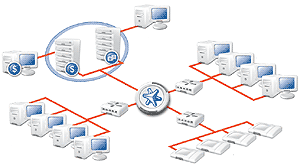
\includegraphics{zorp.png}
  \caption{Példa egy hálózat felépítésének modelljére}
  \label{fig:zorp}
\end{figure}

\subsubsection{Pcap bemutatása}

A számítógép hálózatok területén a pcap (packet capture) biztosít egy
alkalmazásprogramozási felületet (API) a hálózati forgalom rögzítésére.
Unixon alapuló rendszerekben a libcap könyvtár, Windows-os rendszerekben
pedig a WinPcap implementálja.

A pcap API C nyelven készült, más nyelvek wrapper-t használnak hozzá,de maga
a libcap vagy a WinPcap sajnos nem biztosítanak saját wrapper-t.
A libcap és a WinPcap rengeteg nyílt forráskódú és kereskedelmi forgalomban
kapható hálózati szoftverhez biztosítja a csomagrögzítő és szűrő motort, például
hálózat monitorozó eszközök, forgalom generátorok, hálózati behatolást detektáló
rendszerek.

Az elkapott csomagok fájlokba rögzíthetőek és a rögzített csomagok fájlból kis is
olvashatóak.Libcap vagy WinPcap használatával olyan programok készíthetőek melyek a
hálózati forgalomból elkapott csomagokat analizálni képesek, vagy már az előre
rögzített csomagokat fájlból kiolvasva tudják azokat analizálni.

Libcap és WinPcap által használt formátumban elmentett fájlokat például
tcpdump, Wireshark vagy CA NetMaster nevű programokkal tudjuk felhasználni.
A jellemző fájl kiterjesztés a .pcap, de használatban van a .cap és a .dmp
kiterjesztés is.

A .pcap fájl használata egyszerű és sok program képest ezt kezelni.
Előnyként említhető, hogy a ki és bemenő adatcsomagokat is képes kezelni.

Programok melyek a libcap-et/WinPcap-et használnak:

\begin{itemize}
    \itemsep0em
        \item tcpdump
        \item ngrep
        \item Wireshark
        \item Snort
        \item Nmap
        \item Kismet
        \item McAffe
        \item Scapy
\end{itemize}

Wrapper könyvtárak libcap-hez és WinPcap-hez:
\begin{itemize}
\itemsep0em
        \item Perl: Net::Pcap
        \item Python: python-libcap, Pcapy
        \item Ruby: PacketFu
        \item Tcl: tclpcap, tcap, pktsrc
        \item Java: jpcap, jNetPcap, Jpcap,Pcap4j
        \item .Net: WinPcapNet, SharpPcap, Pcap.Net
\end{itemize}

A fájl rendelkezik egy globális header-rel, amely globális információkat
tartalmaz és az azokat követő nulla vagy több rögzített rekordot minden egyes
rögzített csomaghoz:
\\

\begin{tabular}{|l|l|l|l|l|l|l|}
\hline
    Global & Packet & Packet & Packet & Packet & Packet & Packet\\
    Header & Header & Data & Header & Data & Header & Data\\
\hline
\end{tabular}
...
\\

Global Header felépítése:

\begin{lstlisting}
typedef struct pcap_hdr_s {
        guint32 magic_number;
        guint16 version_major;
        guint16 version_minor;
        gint32  thiszone;
        guint32 sigfigs;
        guint32 snaplen;
        guint32 network;
        } pcap_hdrq_t;
\end{lstlisting}
        
\begin{itemize}
\itemsep0em
        \item magic\_number: fájl formátum és a byte rendezés detektálásra használt
        \item version\_major, version\_minor: fájlformátum verziószáma
        \item thiszone: a következő csomag header időbélyegében a helyi időzóna és
a GMT (UTC) közötti idő korrekciója másodpercekben
        \item the correction time in seconds between GMT (UTC) and the local
timezone of the following packet header timestamps
        \item sigfigs: időbélyeg pontossága
        \item snaplen: „snapshot length”
        \item network: kapcsolati réteg header típusa, csomag elején lévő header
típusát specializálja
\end{itemize}

Record (Packet) Header felépítése:

\begin{lstlisting}
typedef struct pcaprec_hdr_s {
    guint32 ts_sec;
    guint32 ts_usec;
    guint32 incl_len;
    guint32 orig_len;
    } pcaprec_hdr_t;
\end{lstlisting}

\begin{itemize}
\itemsep0em
    \item ts\_sec: dátum és idő amikor a csomagot elkaptuk
    \item ts\_usec: a szokásos pcap fájlokban a csomag elkapásának ideje
ezredmásodpecben
    \item incl\_len: az elkapott csomagnak a fájlba mentett adat byte-jainak a
száma
    \item orig\_len: az elkapott csomag hossza a hálózaton
\end{itemize}

\subsubsection{TcpForwarder bemutatása}

Jelenleg a cég rendelkezik egy TcpForwarder nevű eszközzel ami képes adott átmenő kapcsolatok átirányítására a megadott ip címek és portok alapján, illetve ezen kapcsolatokat a Zorp-pal együttműködve rögzíteni illetve visszajátszani.

Azonban a TcpForwarder nem nyílt forráskódú! A cég nem adott ki belőle publikus verziót mint mondjuk a Zorp-ból.

Ez a megvalósítás C++ nyelven készült, de nem minden esetben használható a megfelelően ezért szükség lehet ennek a rendszernek az áttervezésére és javítására.

Az eszköz az adattároláshoz négy darab fájlt használ.
Külön külön elmenti a szerver és kliens oldal adatait kimenő és bemenő irányban, illetve egy kontroll fájlban az egész folyamatot, hogy mi milyen sorrendben történt amit később csak
visszaolvas.

A rendszer felépítése kétféleképpen ábrázolható:

\begin{figure}[h]
  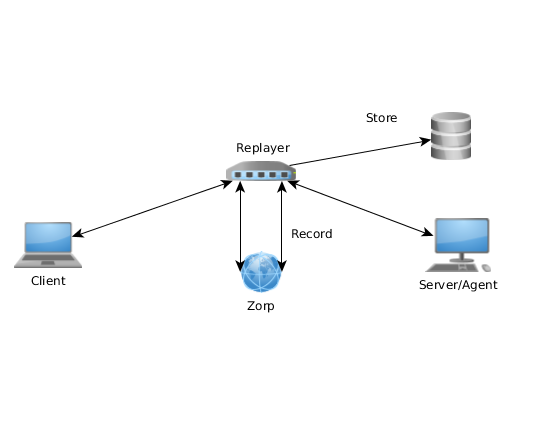
\includegraphics[width=10cm,height=10cm,keepaspectratio]{record.png}
  \caption{Rögzítés TcpForwarderrel}
  \label{fig:record}
\end{figure}

A második ábrán (\ref{fig:record}.) egy olyan hálózatnak a topológiája látható, amelyre a forgalmak rögzítése közben szükség van.
Ilyen módban szükség van egy kliens és egy szerver gépre, egy adattároló eszközre, a Zorp tűzfalra és egy hálózati eszközre ami megteremti a kapcsolatot a többi eszköz között.

A forgalom oda-vissza működik, a kliens géptől elindulva áthaladva a TcpForwarder-en keresztül megérkezik a kapcsolat a tűzfalba, ez után ismét a TcpForwarder-en át tovább halad a szerver gép felé.

Az aktuális beállításainknak megfelelően pedig megtörténik a kapcsolat rögzítése.

(Kliens) <-> (TcpForwarder) <-> (Zorp) <-> (TcpForwarder) <-> (Szerver)
Ez a két TcpForwarder ugyanazt az eszközt jelenti.

Ez a felépítés egy valós tesztkörnyezet alapja lehet, ahol már ténylegesen tesztelhetjük a Zorp-ra épülő eszközt, viszont a szakdolgozatomban elkészült rendszer bemutatására ennél egyszerűbb struktúrát alkalmaztam.

A TcpForwarder másik üzemeltetési módja a már előre rögzített kapcsolat visszajátszására szolgál.

Ennek szemléltetésére az alábbi ábra szolgál: (\ref{fig:replay}.)

\begin{figure}[h]
  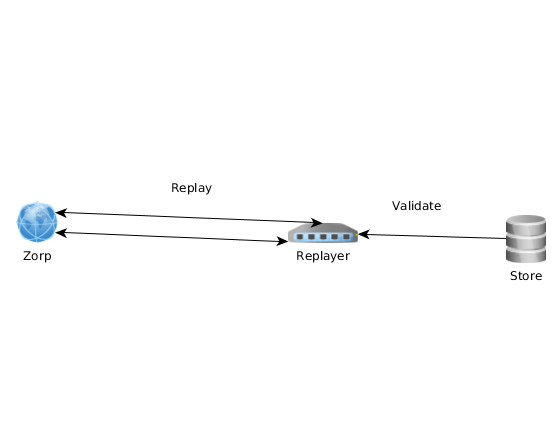
\includegraphics[width=10cm,height=10cm,keepaspectratio]{replay.png}
  \caption{Kapcsolat visszajátszása TcpForwarder-rel}
  \label{fig:replay}
\end{figure}

A visszajátszás esetében már nincs feltétlen szükségünk a kliens és szerver gépekre.
Minimális hálózat felépítéséhez elegendő egy a tűzfalat futtató gép és az azon tárolt kapcsolat. Ilyenkor ezen a gépen indítva a TcpForwarder-t a megfelelő konfigurációs beállításokkal vissza tudjuk játszani a Zorp-on keresztül a meglévő kapcsolatot.
(TcpForwarder) <-> (Zorp)

A TcpForwarder konfigurálásához, egy .ini kiterjesztésű konfigurációs fájl szolgál.
Ebben a fájlban van definiálva a TcpForwarder számára, hogy milyen ip címekről milyen porton figyeljen a bejövő kapcsolatokra, illetve ezeket milyen címre és porton keresztül továbbítsa. Ez megtörténik a kliens és a szerver felőli irányból is.

A zorp/szerver/kliensek címei és portjai egy ini fájlban vannak rögzítve.
Az „in” rész jelenti az elfogadott bejövő kapcsolat, az „out” rész pedig a
TcpForwarder cél címei és portjai.

Példa fájl:
\begin{lstlisting}
[client]
in_address = "any"
in_port = 2209

out_address = "1.1.1.1"
out_port = 2222

[server]
in_address = "any"
in_port = 2210

out_address = "1.1.1.1"
out_port = 23
\end{lstlisting}

A "client" in\_address és in\_port jelenti, hogy a TcpForwarder milyen ip címekről és milyen porton várja, hogy kliensek csatlakozzanak hozzá.
A csatlakozott klienseket a "client" out\_address és out\_port-ján továbbítja a Zorp-ot futtató gép felé, ahol a Zorp a "server" in\_port-ját figyeli.
A TcpForwarder a Zorp felől érkező kapcsolatokat a "server" out\_address és out\_portja felé továbbítja.

Az alábbi ábrán (\ref{fig:streams}.) látható, hogy a fent leírt részegységek miként kapcsolódnak össze:
\begin{center}
\begin{figure}[h]
  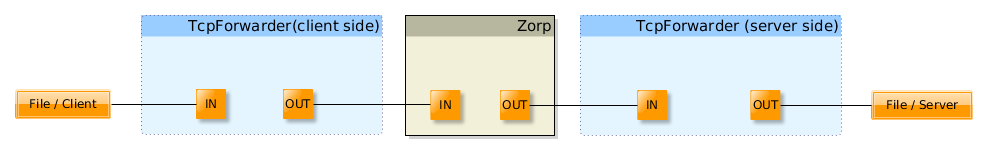
\includegraphics[width=1.15\textwidth,height=4cm]{streams.png}
  \caption{A kliens, TcpForwarder, Zorp és szerver kapcsolata}
  \label{fig:streams}
\end{figure}
\end{center}
\newpage
Ha a bekonfigurált Zorp és TcpForwarder segítségével külön szeretnénk rögzíteni egy kapcsolatot vagy épp visszajátszani egy már előre felvettet akkor azt a következőképpen tehetjük meg.

Rögzítéshez a TcpForwarder futtatható állományát kell indítanunk az alábbi paraméterekkel miután a mappastruktúrában beléptünk a TcpForwarder mappájába:

\begin{lstlisting}
./TcpForwarder record data_folder config.ini
\end{lstlisting}

Ez a parancs a TcpForwardert "record" módban fogja nekünk elindítani. A kapcsolaton keresztül felvett adatokat a "data\_folder" nevű mappába fogja eltárolni, illetve a "config.ini" fájl alapján fogja irányítani a kapcsolatokat.

Miután ez elindult, annyi dolgunk van csak, hogy áthajtunk egy kapcsolatot a konfigurációnak megfelelő ip címre az adott porton.
Ha a kapcsolat lezárult a TcpForwarder is automatikusan megáll.

Visszajátszáshoz az alábbi parancsot használhatjuk:

\begin{lstlisting}
./TcpForwarder replay data_folder config.ini
\end{lstlisting}

Értelem szerűen ebben az esetben a TcpForwarder visszajátszó módban indul, a "data\_folder" mappából olvassa fel a visszajátszandó kapcsolat adatait, és a "config.ini" szerint fog irányítani.

\section{Hasonló célú rendszerek}

Következő lépésként megvizsgáltam, hogy milyen hasonló célú szoftverek, illetve
szoftvercsomagok érhetők el mind nyílt forrású formában, mind pedig kereskedelmi forgalomban.

Erre azért volt szükség, hogy pontosabb képet kapjak a jelenleg fellelhető megoldásokról, és munkám során az így szerzett pozitív és negatív tapasztalatokat eredményesen hasznosíthassam.
Kereséseim során számos kész megoldást találtam, viszont ezek között nem akadtam olyan eszközre amely megfelelne a cégem által támasztott igényeknek.

Vannak olyan eszközök melyek arra specializálódtak, hogy a hálózati forgalmat megfigyelhessük az adatcsomagok szintjén. Vagy akár ezek módosítására is képesek legyünk.

Például az alábbi két eszköz is ilyen:
\begin{itemize}
    \item TCPDUMP \cite{website:tcpdump}
        
        A tcpdump egy általános, ingyenes (BSD license) csomag ellenőrző eszköz. Karakteres felületen lehetővé teszi, hogy láthatóvá váljanak a TCP/IP és más csomagok is, melyeket a hálózaton keresztül küldünk illetve fogadunk.
        
        Előnyei közé tartozik, hogy a legtöbb Unix alapú operációs rendszeren működik, illetve létezik Windows-os megvalósítása is WinDump néven.

    \item Wireshark \cite{website:wireshark}
        
Másik hasonló, de már fejlettebb eszköz a Wireshark nevű ingyenes program.

Ez a program szintén a hálózaton továbbított csomagok megfigyelésére való, akárcsak a tcpdump, viszont ez már rendelkezik egy grafikus felülettel és néhány egyéb rendezési illetve szűrési beállítással.

A Wireshark mind Unix mind Windows-os környezetben használható.
A tcpdump-pal szembeni előnyei ellenére, sajnos ez az eszköz is csak a csomagok illetve a hálózat ellenőrzésére használható.
        
\end{itemize}

Az általam fellelt eszközök másik csoportja a hálózatok tesztelésére szakosodott, oly módon,
hogy az azokon átmenő kapcsolatok számát próbálják felmérni vagy az adatáteresztő képességüket.

Ilyen eszköz például:
\begin{itemize}
\item Iperf \cite{website:iperf}

Ez szintén egy ingyenes hálózat tesztelő eszköz, amely képes TCP illetve UDP adatfolyamokat generálni a hálózaton, amivel mérhetővé válik annak teljesítménye.
\end{itemize}

Kereséseim során fellelt eszközök, csak részben fednék le a cég által felállított követelményeket.
A jelenlegi helyzetben nem elég csak rögzíteni a hálózaton továbbított adatcsomagokat, vagy épp csak a hálózat teljesítményét tesztelni.
Képesnek kell lenni arra, hogy a Zorp tűzfalra épített rendszereken meg tudjuk mondani, hogy valós nagyvállalati környezetben adott hálózati protokollok esetében a rendszer mennyire képes ellátni a feladatát és ezt milyen minőségben teszi.

Az általam fejlesztett megoldás viszont a TcpForwarder segítségével konkrétan erre a kérdésre próbál választ adni.

\section{A rendszer tervezése}
\subsection{Követelmények}
Elsődleges szempont volt, hogy az időnként szükséges teljesítménytesztek lebonyolításánál a lehető legtöbb feladatot automatizálhassuk és a lehető legkönnyebben elvégezhetőek legyenek a műveletek.

A teszt rendszer tervezésekor az alábbi követelmények lettek megállapítva:
\begin{itemize}
    \itemsep0em
        \item Könnyű konfigurálhatóság
        \item Központosított moduláris rendszer
        \item Automatikus logolás
        \item Könnyű bővíthetőség
\end{itemize}

\subsection{Modulok}
Maga az egész tesztrendszer magába foglalja a TcpForwarder-t is ugye, de annak részletes bemutatására nem térnék ki, mert az már egy előzőleg elkészült rész.

A szakdolgozat keretein belül fejlesztett tesztrendszer magját alkotó rhino fantázia névre keresztelt eszköz az alábbi főbb modulokból áll:

\begin{enumerate}
    \itemsep0em
        \item Configurations
        \item Agents, Clients
        \item Network
        \item Pool(Thread Pool)
\end{enumerate}

\subsubsection{Configurations}

A rendszer "configurations" mappájában olyan .config kiterjesztésű fájlokat tárulunk, melyekben előre definiálhatóak az eszköz által létrehozott Clients és Agents tulajdonságai, illetve a Clients által végrehajtott műveletek paraméterezhetőek.

\subsubsection{Agents, Clients}

Az Agents és Clients modulok felelősek a hálózati réteg elindítására, a konfigurációk inicializálására, illetve a kapcsolat fenntartására a kontroller modullal.

A kliensek tekintetében a rendszer rendelkezik egy BaseClient elnevezésű interface-szel, amit minden egyes kliensnek implementálnia kell amit a későbbiekben létrehoznánk.

\subsubsection{Network}
A Network modul felelős a hálózat fenttartásáért, a kapcsolatok kezelésére a csatlakozott kliensekkel.
    
\subsubsection{Pool(Thread Pool)}

A rendszer ezen modulja felelős a szálkezelésért.
Az elindított és beregisztrált kliensek vezérlését végzi, a kliensek feladatait indítja, ütemezi.

\subsection{Választott technológiák}

A feladat megtervezése után a következő lépés a technológia kiválasztása volt, melyben a megvalósítást véghezvihetem.

Munkahelyi feladataim illetve a Zorp Python-os háttere miatt hamar erre a programozási nyelvre esett a választás.

A fejlesztés illetve a dolgozat elkészítése során verziókövetésre Git-et \cite{website:git}, Latex-et Gummi-val \cite{website:gummi}, illetve az ábrák szerkesztéséhez Yed-et \cite{website:yed} használtam.
A TcpForwarder esetleges módosításához Qt-t \cite{website:qt} használtam.
A leadott rendszert egy virtuális gépben helyeztem el, amit Oracle VM VirtualBox-ban készítettem és használtam. \cite{website:vbox}

A virtuális gépen egy Linux Mint 17(qiana) fut. \cite{website:linuxmint}

Magát a keretrendszert elindító komponensek pedig Bash szkriptekben készültek.

\subsubsection{Python \cite{book:python}}


A Python egy magas szintű, általános célú programozási nyelv, melynek elsődleges filozófiája a fejlesztési feladatok megkönnyítése és produktivitásának növelése, még ha ez a sebesség rovására is megy.

A Python egy szkript nyelv, úgynevezett interpreteres nyelv, mely nem igényel például a C/C++ kódokhoz hasonlóan fordítót, a megírt kódok azonnal futtathatóak, nincsenek elválasztva egymástól a forrás és tárgykódok.

\section{A fejlesztés részletei}

\subsection{Architekturális terv}

Az alábbi ábrán tekinthető meg a keretrendszer architekturális terve: (\ref{fig:load_generator}.)

\subsection{Fejlesztési napló}
\begin{enumerate}
    \itemsep0em
        \item Környezet kiépítése
        
            Első feladatom az volt, hogy a saját virtuális gépemen egy megfelelő környezetet építsek ki a Zorp installálásával. A TcpForwarder lefordítása után a saját környezetemben be kellett konfiguráljam a hálózatnak megfelelően, hogy együtt tudjon működni a Zorp-pal.
            
        \item A keretrendszer alapjai
        
        Megvalósításra került a rendszer alapja, elkészültek a Clients, Agents modulok.
        
        \item Bővítés
        
        A parancssori utasítások bővültek, a Network és ThreadPool modulok implementálása megtörtént.
        
        \item TcpForwarder hívása
        
        A TcpForwarder bekötése a rendszerbe és ezen keresztül történő irányítása.
        
        \item Tesztelés
        
        Telnet kliens implementálása a rendszerbe, valódi környezetben és terméken történő tesztelés.
        
\end{enumerate}

\subsection{Modulok részletes bemutatása}

A továbbiakban szeretném részletesen bemutatni a keretrendszer moduljait.

\subsubsection{Configurations} \label{sssec:configurations}

A konfigurációkat egy egyszer json fájlban tudjuk definiálni, amit később a klienseknél tetszőlegesen felhasználhatunk.

Ennek a konfigurációs fájlnak mindenképp tartalmaznia kell a következőket:
\begin{itemize}
    \itemsep0em
        \item Szimulált kliensek számát
        \item Kliens nevét a betöltéshez és inicializáláshoz
        \item A teszt típusát
        \item Tetszőleges paramétereket a teszt metódusokhoz
        \item A teszt metódus nevét amit a kliens végrehajt majd
\end{itemize}

Az alábbi kódrészleten egy példát láthatunk mely a kliensek viselkedését és tulajdonságait hivatott tartalmazni:

\begin{lstlisting}
{
 "command": "set_test_config",
 "simulate_client_number": 4,
 "client_name": "rhino.clients.exampleclient.ExampleClient",
 "test_type": "INFINITE",
 "time": 1234,
 "parameters": {
        "server_address":"1.1.1.1",
        "another_parameter":"value"
 },
 "test_methods": [
     {
         "method_name": "my_test_method_with_one_parameter",
         "method_execution_number": 1,
         "method_params": [
             "param1"
         ]
     },
     {
         "method_name": "my_test_method",
         "method_execution_number": 1,
         "method_params": []
     },
     {
         "method_name": "my_test_method_with_two_parameters",
         "method_execution_number": 1,
         "method_params": [
             "param1",
             "param2"
         ]
     }
 ]
}
\end{lstlisting}

\begin{itemize}
    \itemsep0em
        \item "simulate\_client\_number": Itt adhatjuk meg, hogy párhuzamosan hány darab klienst hozzunk létre
        \item "client\_name": Ez a paraméter a már előre definiált kliens fajtáját jelenti, ezt igényeinknek megfelelően a saját kliensünkkel kiválthatjuk.
        \item "test\_type": Itt a teszt futásának fajtáját adhatjuk meg, ami jelen esetben három féle lehet: SEQUENCE, INFINITE, TIME\_LIMITED
        \item "parameters": Az itt megadott paraméterek átadódnak majd az elkészült klienseknek.
        \item "test\_methods": Ebben a paraméterben egy listát adunk át a rendszernek, ahol tetszőleges mennyiségű teszt metódust adhatunk meg.

        A lista elemeinek a következő felépítésnek kell megfelelniük:
        \begin{itemize}
            \itemsep0em
                \item "method\_name": Ez a paraméter a kliensben definiált tesztmetódus nevét tartalmazza ami majd le fog futni.
                \item "method\_execution\_number": A tesztmetódus hány alkalommal fusson le.
                \item "method\_params": Itt szintén egy listát kell megadnunk, ami a meghívott teszt metódusnak megfelelően megegyező mennyiségű paramétert tartalmaz string-ek formájában.
        \end{itemize}

\end{itemize}

\subsubsection{Agents - agents.py}

Ebben a modulban két féle osztály van implementálva.

A rendszer indításakor parancssori argumentumként kapja meg a kontroller, hogy az aktuális indítás kliens, vagy szerver módban történt, és ennek megfelelően vagy ServerAgent vagy ClientAgent ként fog futni.

A ServerAgent által megvalósított metódusok, az alábbi osztálydiagramon láthatóak: (\ref{fig:serveragent_class}.)

    \begin{figure}[h]
      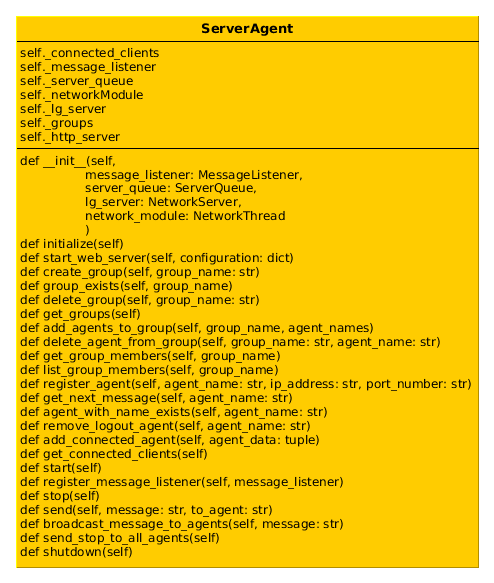
\includegraphics[width=13cm, keepaspectratio]{serveragent_class.png}
      \caption{ServerAgent }
      \label{fig:serveragent_class}
    \end{figure}

Ebből az osztályból létrejött objektum az alábbi adattagokat tartalmazza:
\begin{itemize}
    \itemsep0em
        \item Rendelkezik a self.\_connected\_clients listával, ami a csatlakozott kliensekről tárol (név , IP cím) párokat.
        \item Rendelkezik egy self.\_message\_listener adattaggal ami egy MessageListener objektumot tárol.
        \item A self.\_server\_queue adattagba egy ServerQueue objektumot tárol, ami olyan üzeneteket tartalmaz amiket mindenképp ki kell küldeni a csatlakozott klienseknek.       
        \item A self.\_networkModule adattag egy NetworkThread-et vesz át.
        \item A self.\_lg\_server adattag egy NetworkServer objektumot vesz át.
         \item A self.\_groups egy lista, ami a futás közben készített csoportokat tartalmazza.
        \item A self.\_http\_server pedig egy a későbbiekben esetleges webes felülethez szükséges szerver objektumot tartalmazza
\end{itemize}

A ServerAgent osztály felelős azért, hogy biztosítsa a kliensek koordinálását, azokról információt szolgáltasson ha szükség van rá.
Képes csoportokba szervezni a klienseket, a csoportokat módosítani/törölni.

A másik osztály amely itt kapott helyet az a ClientAgent, aminek az osztálydiagramja az alábbi ábrán látható (\ref{fig:clientagent_class}.)

    \begin{figure}[h]
      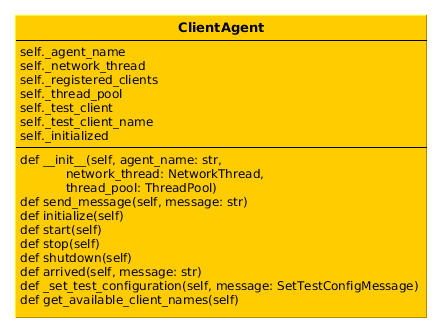
\includegraphics[width=13cm, keepaspectratio]{clientagent_class.png}
      \caption{ClientAgent}
      \label{fig:clientagent_class}
    \end{figure}
    
\begin{itemize}
    \itemsep0em
        \item Rendelkezik egy saját névvel, ez egy egyszerű string típus
        \item Rendelkezik egy self.\_network\_thread adattaggal ami egy NetworkThread-et tárol
        \item Egy listában tárolja a regisztrált klienseket self.\_registered\_clients = []
        \item A self.\_thread\_pool adattagban egy ThreadPool objektumot tárol
        \item A self.\_test\_client és a self.\_test\_client\_name adattagok egy kliens példányról tárolnak információt
         \item  A self.\_initialized adattag jelzi, hogy a teszt konfiguráció be lett-e állítva
         Ez 1 értéket vesz fel ha a kliens elindult, különben 0.
\end{itemize}
    
\subsubsection{Clients - /clients}

A rendszerben lehetőségünk van definiálni számtalan különböző klienst a rendszer clients nevű mappája alá.

Az itt létrehozott kliensek mindegyikének implementálnia kell az alábbi diagramon látható interfészt: (\ref{fig:baseclient}.)

\begin{figure}[h]
  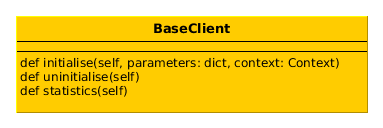
\includegraphics[width=13cm, keepaspectratio]{baseclient.png}
  \caption{BaseClient}
  \label{fig:baseclient}
\end{figure}

A kliensek felépítésének egyszerű példáját, egy az alább látható példa kód segítségével szeretném bemutatni:


\begin{lstlisting}[language=Python]
@implements(BaseClient)
class ExampleClient:
    def __init__(self):
        pass

    @test_method
    def my_test_method(self):
        print("my_test_method has been called")

    @test_method
    def my_test_method_with_one_parameter(self, str_param: str):
        print("my_test_method_with_one_parameter has been called")

    @test_method
    def my_test_method_with_two_parameters(self, str_param: str, str_param2: str):
        print("my_test_method_with_two_parameters has been called")

    def initialise(self, parameters: dict, context: Context):
        print('Initialized with parameters:', parameters)

    def uninitialise(self):
        pass

    def statistics(self) -> dict:
        return {'stat_param1': randint(0, 234),
                'stat_param2': randint(0, 3000),
                'stat_param3': randint(0, 300),
                'stat_param4': randint(0, 35),
                'stat_param5': randint(0, 799)
               }
\end{lstlisting}

Láthatjuk, hogy a kódrészlet elején a @implement(BaseClient) sorral jelöljük, hogy a BaseClient interfészt fogjuk most megvalósítani.

Az interfész initialise, uninitialise és statistic metódusának mindenképp szerepelnie kell saját kliens osztályunkban is, viszont azok tartalma és képességeik csak attól függenek, hogy mi mit teszünk beléjük.

Jelenleg a statisztikát szolgáltató metódus is csak véletlenszerű adatokból felépített eredménnyel tér vissza.

Ahogy ebben az ExampleClient osztályban is látható, a @test\_method jelzéssel felvihetünk további metódusokat, amiket az osztályhoz tartozó már korábban részletezett konfigurációs fájlban tetszés szerint paraméterezhetünk és indíthatunk akárhány alkalommal.

Az itt definiált klienseket a keretrendszer konfigurációs fájljába is be kell kötnünk, hogy elérhetővé váljanak futás közben.

Ez a konfigurációs fájl a virtuális gép /home/gabor/load\_generator/rhino/ elérési út alatt található rhino.config fájl.

Egy lehetséges példa a rhino.config fájl tartalmára:
\begin{lstlisting}
        {
            "log_level" : 2,
            "log_file": "rhino.log",
            "web_server": "True",
            "web_server_listen_port":8080,
            "web_directory":"www",
            "clients": [
                "rhino.clients.exampleclient.ExampleClient",
            ]
        }
\end{lstlisting}

Jelen esetben az alábbi attribútumok lényegesek a mi szempontunkból:
\begin{itemize}
\itemsep0em
    \item "log\_level": Ez a paraméter felelős a rendszer futás közbeni logolás mértékének beállításáért
    \item "log\_file": Ezzel a paraméterrel egy string segítségével adhatjuk meg, hogy milyen elérési úton illetve milyen nevű fájlba mentődjenek a log üzenetek.
    
    \item "cliens": Az itt látható lista az, amelybe szükséges az általunk definiált kliensek bekötése.
    
    Példánk alapján ez a bejegyzés azt jelenti, hogy a rhino/clients/ mappában az exampleclient.py kiterjesztésű fájlban az ExampleClient osztályt szeretnénk elérni.
\end{itemize}

\subsubsection{Network}

A network modul alatt az alábbi osztályok lettek implementálva, melyek működése asszinkron módon történik, a NetworkThread osztály kivételével.

\begin{itemize}
    \itemsep0em
        \item NetworkThread (\ref{fig:networkthread}.)
            \begin{figure}[h]
              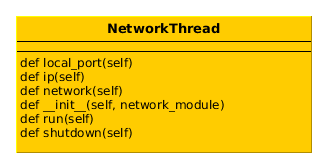
\includegraphics[keepaspectratio]{networkthread.png}
              \caption{NetworkThread}
              \label{fig:networkthread}
            \end{figure}
            
            A NetworkThread osztály felelős a hálózati szálak kezeléséért.

            Indíthat, megállíthat forgalmakat.
            
            Igény esetén képes visszatérni ip címmel és port számmal.
            
            
        \item NetworkServer (\ref{fig:networkserver}.)
            \begin{figure}[h]
              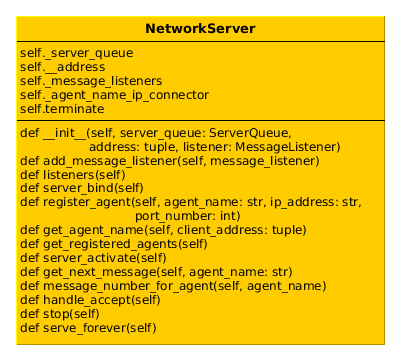
\includegraphics[width=13cm, keepaspectratio]{networkserver.png}
              \caption{NetworkServer}
              \label{fig:networkserver}
            \end{figure}
   
            Az osztály adattagjai:
            \begin{itemize}
                \itemsep0em
                    \item self.\_server\_queue adattag egy ServerQueue objektumot vesz át.
                    \item self.\_\_address ez az adattag (ip, port) párokat tartalmaz.
                    \item self.\_message\_listeners adattag egy lista, amelybe MessageListener objektumokat tárolunk.
                    \item self.\_agent\_name\_ip\_connector egy dict adattag, amiben kulcsként (ip\_address, port\_number) párokat és a hozzá tartozó agent-ek nevét tároljuk.
                    \item self.terminate logikai változó.
            \end{itemize}
            
            A NetworkServer osztály felelős hálózati kommunikáció lebonyolításáért.
            A listener-ek kezeléséért, a szerver bind-olásáért, képes klienseket regisztrálni, róluk információt kérni.
            Üzeneteket kezel, szerverek indítását/megállítását végzi.
            Szerver

        \item NetworkClient (\ref{fig:networkclient}.)
            \begin{figure}[h]
              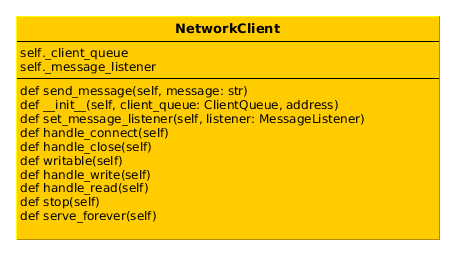
\includegraphics[width=13cm,keepaspectratio]{networkclient.png}
              \caption{NetworkClient}
              \label{fig:networkclient}
            \end{figure}
            
            Az osztály adattagjai:
            \begin{itemize}
                \itemsep0em
                    \item self.\_client\_queue adattag egy ClientQueue objektumot kap, ami az üzenetek kezelését végzi.
                    \item self.\_message\_listener egy MessageListener objektumot tartalmaz.
            \end{itemize}
            
            A NetworkClient osztály feladata az üzenetek kezelése, fogadása a kliensek felől illetve továbbítása azok felé.
            
        \item ServerHandler (\ref{fig:serverhandler}.)
            \begin{figure}[h]
              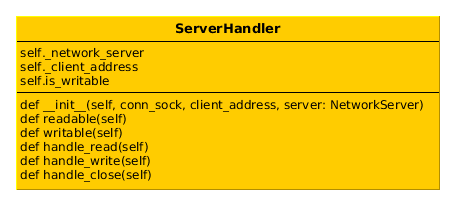
\includegraphics[width=13cm,keepaspectratio]{serverhandler.png}
              \caption{ServerHandler}
              \label{fig:serverhandler}
            \end{figure}
            
            Az osztály adattagjai:
            \begin{itemize}
                \itemsep0em
                    \item self.\_network\_server ez az adattag egy NetworkServer objektumot tartalmaz.
                    \item self.\_client\_address kliens címét tároló adattag.
                    \item self.is\_writeable logikai változó.
            \end{itemize}

        A ServerHandler osztály felelős a csatlakozott kliensek kapcsolatának kezeléséért.
            
\end{itemize}
\newpage
\subsubsection{Pool}

Ebben a modulban az alábbi osztályok lettek implementálva:
\begin{itemize}
    \itemsep0em
        \item ThreadPoolInterface
        
\begin{lstlisting}[language=Python]
@interface
class ThreadPoolInterface:

    def initialise(self, with_test_client_name: str, with_test_config: SetTestConfigMessage=None, with_thread_number=1):
        pass

    def start_executors(self):
        pass

    def stop_executors(self):
        pass

\end{lstlisting}

Ez az osztály egy alap interfészt biztosít, ami a későbbiekben a ThreadPool osztályon belül implementálásra került.

        \item ThreadPool (\ref{fig:threadpool}.)
        
        \begin{figure}[h]
              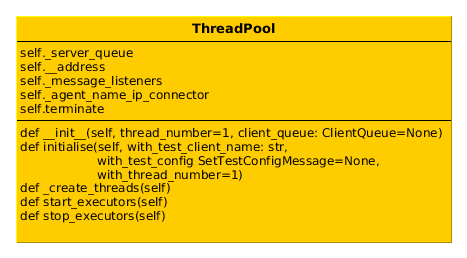
\includegraphics[width=13cm,keepaspectratio]{threadpool.png}
              \caption{ThreadPool}
              \label{fig:threadpool}
            \end{figure}
            \newpage
        Az osztály adattagjai:
            \begin{itemize}
                \itemsep0em
                    \item self.\_thread\_number ez az adattag jelenti, hogy hány szálat fog létrehozni a rendszer.
                    \item self.\_threads az elkészült szálakat ebben a listában tároljuk.
                    \item self.\_running logikai változó, a futást jelzi.
                    \item self.\_test\_config ez az adattag tartalmazza az inicializálás során átvett konfigurációt.
                    \item self.\_test\_client\_name ez az adattag tartalmazza az inicializálás során átvett teszt kliens nevét.
                    \item self.\_context adattag egy Context(client\_queue) típusú objektumot tartalmaz ami az üzenetküldésért és objektumok regisztrálásáért felel.
            \end{itemize}

Ez az osztály felelős a szálak kezeléséért.

A konfigurációnak megfelelően létrehozza az ott megadott mennyiségű szálat, amit majd az ExecutorThread osztálynak átad.

Ezen osztályon keresztül történik a szálakhoz tartozó kliensek feladatainak indítása és megállítása.

        \item ExecutorThread
            \begin{figure}[h]
                  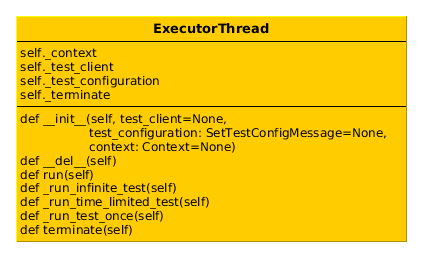
\includegraphics[width=13cm,keepaspectratio]{executorthread.png}
                      \caption{ExecutorThread}
                  \label{fig:executorthread}
            \end{figure}
\newpage
    Az osztály adattagjai:
    
        \begin{itemize}
            \itemsep0em
                \item self.\_context Context típusú objektumot tartalmazó adattag.
                \item self.\_test\_client a konfigurációból átvett kliens nevét tartalmazza.
                \item self.\_test\_configuration a beállított teszt konfigurációt tartalmazza.
                \item self.\_terminate logikai változó.
        \end{itemize}
        
        Az ExecutorThread objektumok feladata, hogy a konfigurációban megadott módon és a paramétereknek megfelelően futtassa a teszt kliensek metódusait.
\end{itemize}

A létrehozott szálak indítása nem szekvenciális módon történik.
Ha legalább 2 szálat létrehoztunk és kiadjuk a parancsot ezek elindítására akkor az összes szál párhuzamos módon egyszerre fog elindulni.
        
\section{Felhasználói dokumentáció}

A következő fejezetben szeretném bemutatni az elkészült keretrendszer és a már meglévő komponensek együttes működését és használatát egy leegyszerűsített rendszeren.

A dolgozatom mellékleteként csatolt virtuális gép tartalma:
\begin{itemize}
    \itemsep0em
        \item A rendszer alapja egy már korábban említett Linux Mint 17-es operációs rendszer
        \item Telepített publikus verziójú Zorp tűzfal, bekonfigurálva
        \item A fejlesztett keretrendszer az aktuális állapotában
        \item Lefordított TcpForwarder, elkészített konfigurációs fájllal
\end{itemize}

\subsection{Rendszer követelmények}

A rendszer indításához az alábbi programot szükséges feltelepíteni egy számítógépre : \cite{website:vbox}

A telepítés után a .vbox kiterjesztésű fájl megnyitásával elindíthatjuk a virtuális gépet.
Arra figyeljünk, hogy a virtuális gépnek szüksége van egy processzor magra, 2GB memóriára illetve 8-10GB háttértárra.

Lehetőleg próbáljuk meg olyan számítógépen elindítani a rendszert ami rendelkezik legalább 2 fizikai maggal rendelkező CPU-val, illetve mindenképp több mint 4GB memóriával rendelkezik(6-8GB ajánlott, a számítógép operációs rendszerének függvényében) a zökkenőmentes futtatás érdekében.

A rendszerben használatos felhasználó név "gabor", a jelszó pedig egy darab "a" betű. Ezek segítségével tudunk majd root jogot szerezni, illetve belépni a rendszerbe a tesztek során.

\subsection{Használat és a működés bemutatása}

A következőkben már egy valósnak mondható forgatókönyv alapján szeretném bemutatni a rendszer működését.

Ahogy a keretrendszer fejlődött, elkészült hozzá egy telnet kapcsolaton alapuló kliens típus, ami az előre elkészített konfigurációs fájlokkal képes automatikus módon a megadott célgépen egy telnet kapcsolatot létesíteni, ezen a kapcsolaton keresztül néhány alap műveletet végrehajtani és ezt közben a TcpForwarder segítségével rögzíteni, illetve visszajátszani.

Ezen konfigurációs fájlok a configurations mappában találhatóak.

Név szerint:
\begin{itemize}
\itemsep0em
\item telnet\_parallel.config: Ez a konfiguráció a "test\_parallel\_telnet" nevű teszt metódust fogja használni, 10 klienst fog elindítani, illetve a tesztmetódust minden egyes kliens 5 alkalommal fogja lefuttatni.
\item telnet\_record.config: Ez a konfiguráció 1 telnet klienst fog létrehozni illetve egy alkalommal fogja lefuttatni a "test\_record" metódust.
\item telnet\_replay.config: Az utolsó konfiguráció pedig a már előre rögzített "example\_connection\_for\_replay" mappa alatt tárolt adatokat fogja 30 alkalommal visszajátszani és validálni.
\end{itemize}


Példámban a "telnet\_parallel.config"-ot fogom használni, mert jelenleg ezekkel a beállításokkal képes a rendszer a legnagyobb terhelést kifejteni, amit ha egy rendszermonitort(System Monitor) elindítunk miközben futtatjuk a klienseket ez jól láthatóvá is válik a processzorhasználaton.

Röviden bemutatnám a példában is használt konfigurációs fájlt, illetve a TelnetClient felépítését.

A "telnet\_parallel.config" konfigurációs fájl tartalma:

\begin{lstlisting}
{
 "command": "set_test_config",
 "simulate_client_number": 10,
 "client_name": "rhino.clients.telnetclient.TelnetClient",
 "test_type": "SEQUENCE",
 "time":2345,
 "parameters": {
        "server_address":"1.1.1.1",
        "user": "gabor",
        "password": "a",
        "another_parameter":"value"
 },
 "test_methods": [
     {
         "method_name": "test_parallel_telnet",
         "method_execution_number": 5,
         "method_params": []
     }
 ]
}
\end{lstlisting}

A TelnetClient osztály diagramja az alábbi ábrán látható (\ref{fig:telnetclient}.):

\begin{figure}[h]
  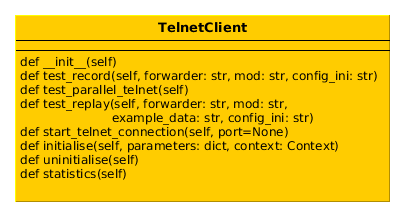
\includegraphics[width=13cm,keepaspectratio]{telnetclient.png}
  \caption{TelnetClient}
  \label{fig:telnetclient}
\end{figure}

Láthatjuk, hogy a BaseClient osztályhoz képest TelnetClient osztályunk már rendelkezik négy darab extra metódussal amik az alábbiak:
\begin{itemize}
\itemsep0em
\item test\_record(self, forwarder: str, mod: str, config\_ini: str)

Ez a metódus vezérli a keretrendszeren keresztül történő kapcsolat rögzítést.

\item test\_parallel\_telnet(self)

Ez az egyszerű metódus a fentebb is látható konfig alapján 10 páldányon keresztül 5-5 alkalommal fog meghívódni, miközben minden egyes alkalommal elindítja a start\_telnet\_connection függvényt.

\item test\_replay(self, forwarder: str, mod: str, example\_data: str, config\_ini: str)

Ezzel a metódussal indíthatjuk a visszajátszást a keretrendszeren keresztül.

\item start\_telnet\_connection(self, port=None)

Ennek a metódusnak a segítségével épít fel a rendszer egy egyszerű telnet kapcsolatot.

\end{itemize}

\begin{enumerate}
\item A már korábban említett VirtualBox \cite{website:vbox} telepítése után indítsuk el a virtuális gépet.
\item  Miután a rendszer elindult és betöltött indítsunk el egy "Terminator"-t. Baloldalt felül található piros négyzetekkel kirakott ikon, vagy az asztalon található indítóikon segítségével.

Ez egy egyszerű karakteres felületű terminál, mint bármelyik Linux operációs rendszeren, csak van néhány plussz hasznos funkciója ami segítségünkre lehet.

A könnyebb kezelhetőség érdekében osszuk fel 4 részre a Terminátor ablakát.
Ezt megtehetjük az alábbi gyorsbillentyűkkel:
\begin{itemize}
\itemsep0em
\item CTRL + SHIFT + E : függőlegesen osztja ketté az ablakot
\item CTRL + SHIFT + O : vízszintesen osztja ketté az ablakot
\end{itemize}
Vagy a Terminátor ablakán jobb egérgombot megnyomva kiválasztjuk a "Split Horizontally/Vertically" opciókat. Ez után ha szeretnénk a könnyebb áttekinthetőség érdekében az egyes kis ablakokat át is tudjuk nevezni.

Ezek után valami hasonlót kell lássunk:
\begin{figure}[h]
      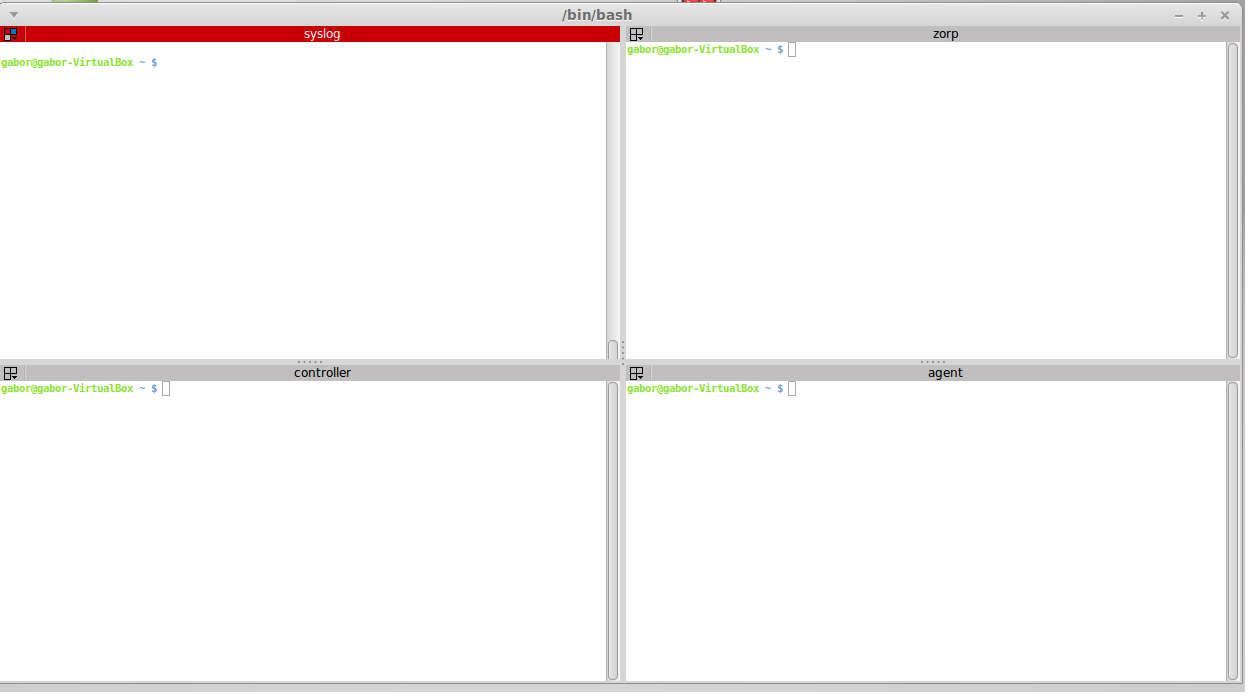
\includegraphics[width=1\textwidth,keepaspectratio]{1.png}
          \caption{Terminator}
      \label{fig:terminator}
\end{figure}

Ez a nézet a későbbiekben segítségünkre lesz, hogy egyszerűbben átlássuk, az éppen futó folyamatokat és azok eredményeit.

\item Következő lépésként ellenőrizzük, hogy az előre beállított hálózati interfész megfelelő ip címmel rendelkezik-e.

Ezt a következő parancs kiadásával tudjuk ellenőrizni, aminek hatására ehhez hasonló kimenetet kell kapnunk:
\begin{lstlisting}[language=bash]
gabor@gabor-VirtualBox ~ $ ifconfig
eth0      Link encap:Ethernet  HWaddr 08:00:27:48:66:19  
          inet addr:192.168.0.100  Bcast:192.168.0.255  Mask:255.255.255.0
          inet6 addr: fe80::a00:27ff:fe48:6619/64 Scope:Link
          UP BROADCAST RUNNING MULTICAST  MTU:1500  Metric:1
          RX packets:76401 errors:0 dropped:0 overruns:0 frame:0
          TX packets:25636 errors:0 dropped:0 overruns:0 carrier:0
          collisions:0 txqueuelen:1000
          RX bytes:89970010 (89.9 MB)  TX bytes:2145449 (2.1 MB)

eth1      Link encap:Ethernet  HWaddr 08:00:27:a0:43:ee  
          inet addr:1.1.1.1  Bcast:1.255.255.255  Mask:255.0.0.0
          inet6 addr: fe80::a00:27ff:fea0:43ee/64 Scope:Link
          UP BROADCAST RUNNING MULTICAST  MTU:1500  Metric:1
          RX packets:0 errors:0 dropped:0 overruns:0 frame:0
          TX packets:248 errors:0 dropped:0 overruns:0 carrier:0
          collisions:0 txqueuelen:1000
          RX bytes:0 (0.0 B)  TX bytes:51681 (51.6 KB)

lo        Link encap:Local Loopback  
          inet addr:127.0.0.1  Mask:255.0.0.0
          inet6 addr: ::1/128 Scope:Host
          UP LOOPBACK RUNNING  MTU:65536  Metric:1
          RX packets:621 errors:0 dropped:0 overruns:0 frame:0
          TX packets:621 errors:0 dropped:0 overruns:0 carrier:0
          collisions:0 txqueuelen:0
          RX bytes:59730 (59.7 KB)  TX bytes:59730 (59.7 KB)
\end{lstlisting}

Számunkra a kérdéses csatlakozó az "eth1" jelölésű. Ennek az "inet addr" címének 1.1.1.1-nek kell lennie.

Ha esetleg nem ezt az ip címet látnánk a csatlakozó mellett, akkor az alábbi parancs használatával állítsuk azt be:

\begin{lstlisting}
gabor@gabor-VirtualBox ~ $ sudo ifconfig eht1 1.1.1.1
\end{lstlisting}

\item Következő lépésként az egyik terminál ablakban adjuk ki a következő parancsot:

\begin{lstlisting}
gabor@gabor-VirtualBox ~ $ tail -f /var/log/syslog
\end{lstlisting}

Ennek eredménye ként ebben az ablakban folyamatosan látni foglyuk, hogy a rendszer milyen üzeneteket logol a különböző programoktól, futó szolgáltatásoktól.

\item Kattintsunk át egy másik ablakba, az előzőt hagyjuk folyamatosan futni.

Következő lépésünkhöz szükség lesz root jogosultságokat szereznünk.
Ezt a következő parancs használatával érhetjük el, aminek kiadása után a rendszer kérni fogja a jelszavunkat ami ahogy már korábban említettem egy darab "a" betű.

Az alábbi kimenethez hasonlónak kell látszania:

\begin{lstlisting}
gabor@gabor-VirtualBox ~ $ su
Password:
gabor-VirtualBox gabor #
\end{lstlisting}

A következő paranccsal a telepített Zorp mappájába ugrunk és ellenőrizzük a mappa tartalmát:
\begin{lstlisting}
gabor-VirtualBox gabor # cd /usr/local/etc/zorp/
gabor-VirtualBox zorp # ls -l
total 24
-rw-r--r-- 1 root root  618 nov   14 16:45 instances.conf
-rw-r--r-- 1 root root  547 márc  26  2015 instances.conf.sample
-rw-r--r-- 1 root root 3710 márc  26  2015 policy.py.sample
-rw-r--r-- 1 root root  987 dec    1 11:10 policy-telnet.py
drwxr-xr-x 2 root root 4096 márc  26  2015 urlfilter
-rw-r--r-- 1 root root 1425 márc  26  2015 zorpctl.conf.sample
\end{lstlisting}

Amire nekünk most szükségünk van az az "instances.conf" és a "policy-telnet.py" fájlok.

Az "instances.conf" fájl tartalma:
\begin{lstlisting}
##################################################
##
## Copyright (c) 2000-2001 BalaBit IT Ltd, Budapest, Hungary
## All rights reserved.
##
##################################################
#
# This file lists the Zorp instances you want to run.
#
# The instance name and arguments _must_ be separated by spaces instead
# of tabs! Otherwise zorpctl will stop working.

#instance  arguments

zorp_telnet --verbose=10 --policy /usr/local/etc/zorp/policy-telnet.py

\end{lstlisting}

Ebben a fájlban tudjuk paraméterekkel ellátni a Zorp futó service-ét.

Jelen esetben a logolást a maximális 10-es értékre állítottuk a "--verbose=" kapcsolóval.
A "--policy" kapcsoló után meg kell adnunk egy elérési utat, ami a saját policy fájlunkhoz vezet, amit a Zorp majd használni fog.

A policy-telnet.py fájl tartalma a következő:

\begin{lstlisting}
# policy.py showing how to use audit policies with startAudit

## Run
# $ telnet localhost -p 2222

from Zorp.Core import *
from Zorp.Telnet import *

config.options.kzorp_enabled = False

InetZone("intnet", "0.0.0.0/0")

def zorp_telnet():
    Service("telnet", TelnetProxy, router=DirectedRouter(SockAddrInet("1.1.1.1", 2210), forge_addr=FALSE))
    Dispatcher(transparent=FALSE, bindto=DBIface(iface="eth1", port=2222, protocol=ZD_PROTO_TCP), service="telnet")

\end{lstlisting}

Ebben a fájlban definiáljuk a saját "zorp\_telnet()" metódusunkat, ami alapján a Zorp működni fog.

Jelen helyzetben a rendszer az 1.1.1.1 ip címen és a 2210-es porton fogja továbbítani az adatokat.
Illetve az eth1-es hálózati interfészen a 2222-es porton pedig várja a csomagokat.

Ha ezek a fájlok rendben vannak, akkor a következő parancs kiadásával elindíthatjuk a Zorp-ot:

\begin{lstlisting}
gabor-VirtualBox zorp # zorpctl start
Starting Zorp Firewall Suite: zorp_telnet#0
gabor-VirtualBox zorp #
\end{lstlisting}

Közben láthattuk a másik ablakban ahol a log változásait figyeljük, hogy a Zorp service elindult.

Ha esetleg módosítani szeretnénk a policy vagy az instance fájlon, akkor a módosítások után az alábbi paranccsal újraindíthatjuk a szolgáltatást, hogy életbe léphessenek a módosításaink:

\begin{lstlisting}
gabor-VirtualBox zorp # zorpctl restart
\end{lstlisting}

Leállítása pedig a stop parancs segítségével történik:
\begin{lstlisting}
gabor-VirtualBox zorp # zorpctl stop
\end{lstlisting}

\item A következő lépés a keretrendszer elindítása lesz.

Ehhez a harmadik terminál ablakban menjünk bele a rhino mappába.

Ez az alábbi parancs kiadásával egyszerűen meg tudjuk tenni, és ha listázzuk a mappa tartalmát akkor ezt a kimenetet kell lássuk:

\begin{lstlisting}
gabor@gabor-VirtualBox ~ $ cd Desktop/load_generator/rhino/
gabor@gabor-VirtualBox ~/Desktop/load_generator/rhino $ ls -l
total 2248
-rwxr-xr-x  1 gabor gabor     117 nov   15 16:00 agent.bash
-rw-r--r--  1 gabor gabor     150 nov   15 15:47 command.test
drwxr-xr-x  2 gabor gabor    4096 dec    1 14:53 configurations
-rwxr-xr-x  1 gabor gabor      77 nov   15 15:55 controller.bash
drwxr-xr-x  2 gabor gabor    4096 nov   15 15:47 doc
drwxr-xr-x  2 gabor gabor    4096 dec    1 14:13 example_connection_for_replay
-rw-r--r--  1 gabor gabor     488 nov   15 15:47 MANIFEST
-rw-r--r--  1 gabor gabor      70 nov   15 15:47 MANIFEST.in
-rw-r--r--  1 gabor gabor 1525093 nov   18 11:52 out.ogv
-rw-r--r--  1 gabor gabor     767 dec    1 14:52 README.txt
drwxr-xr-x 12 gabor gabor    4096 dec    7 19:12 rhino
-rw-r--r--  1 gabor gabor     483 nov   16 13:29 rhino.config
-rw-r--r--  1 gabor gabor  709073 dec    1 14:54 rhino.log
-rw-r--r--  1 gabor gabor    1258 dec    1 14:52 setup.py
drwxr-xr-x  2 gabor gabor    4096 nov   15 15:47 specification
drwxr-xr-x  5 gabor gabor    4096 dec    1 14:53 www
gabor@gabor-VirtualBox ~/Desktop/load_generator/rhino $

\end{lstlisting}

Ugyanezt a műveletet ismételjük meg az utolsó terminál ablakban is.

Az egyik ablakban el tudjuk majd indítani a keretrendszerhez tartozó controller szkriptet, a másik ablakon pedig az agent szkriptet.

Néhány mondatban ismertetném ezen szkriptek tartalmát, és feladatukat.

controller.bash szkript tartalma:
\begin{lstlisting}
#!/bin/bash
python3.4 -m rhino  --mode server -lp 8888 --config rhino.config
\end{lstlisting}

agent.bash:
\begin{lstlisting}
#!/bin/bash
python3.4 -m rhino --name testagent --mode client -lp 8889 -ci 127.0.0.1  -cp 8888 --config rhino.config
\end{lstlisting}

A "controller.bash" szkript feladata egy szerver indítása, amin keresztül irányítani tudjuk a klienseket.

Az "agent.bash" szkript felelős egy teszt kliens elindításáért.

Magyarázat a szkriptekben használt kapcsolókhoz:

\begin{itemize}
\itemsep0em
    \item --config: A betöltött konfigurációs fájl elérési útja.
    \item --mode: Itt kell megadnunk, hogy a rendszert szerver vagy kliens módban akarjuk elindítani [server|client].
    \item --name: Ezzel a kapcsolóval adhatjuk meg az elindított kliensünk nevét. Ha a rendszer kliens módban van elindítva akkor ezt a paramétert mindenképp meg kell adnunk.
    \item -lp: Ez a kapcsoló jelenti, hogy milyen helyi portot használjon a rendszer.
    \item -ci: Ezt a kapcsolót kliens módban kell megadnunk, azt jelenti, hogy a kontroller milyen ip-címen dolgozik.
    \item -cp: Ez a kapcsoló szintén a klienshez tartozik. Azt a portot kell itt megadnunk ahol a kontroller figyel.
\end{itemize}

\item Miután megismertük a két szkript feladatát és tartalmát, az egyik üres terminál ablakban elindíthatjuk a "controller.bash", a másik ablakban pedig az "agent.bash" szkripteket.

Az "agent.bash" szkript elindítása után nem jelenik meg semmi a kimeneten, csak ha a kontrollerrel valamilyen feladatot hajtunk végre a kliensekkel.

A kontroller indításához adjuk ki az alábbi parancsot, majd ennek a képernyőnek kell megjelenni a terminálunkban:

\begin{lstlisting}
gabor@gabor-VirtualBox ~/Desktop/load_generator/rhino $ ./controller.bash
(Lg) >
\end{lstlisting}

Ez a felület jelenti azt, hogy a program elindult.

Itt kiadva a "help" parancsot, a rendszer segítségképp kilistázza, hogy milyen parancsokkal rendelkezik:

\begin{lstlisting}
(Lg) > help

Documented commands (type help <topic>):
========================================
add_agents_to_group    help                   start           
create_group           list_group_members     start_statistics
delete_group           list_groups            stop            
get_available_clients  load_file              stop_statistics
get_client_info        set_group_test_config
get_connected_agents   set_test_config      

Undocumented commands:
======================
exit  version

(Lg) >

\end{lstlisting}

Ahogy a kimeneten is látszik a rendszerben vannak dokumentációval rendelkező parancsok, amiket a leírását a "help <parancs>" segítségével megkaphatunk.

Például ha az "add\_atents\_to\_group" parancsra vagyunk kíváncsiak akkor az alábbi parancs kiadása után ezt a kimenetet kapjuk:

\begin{lstlisting}
(Lg) > help add_agents_to_group
Add agents to group. add_agents_to_group <group name> <agents separated with comma>
(Lg) >
\end{lstlisting}

A parancsok használatának megkönnyítése érdekében a rendszer rendelkezik parancs kiegészítéssel a TAB billentyű megnyomásával, akárcsak egy hagyományos terminál esetében.

Jelen környezetben egy teszt klienst fogunk indítani, amivel szemléltetni szeretném a keretrendszer működését és az alábbi parancsok használatát:
\begin{itemize}
\itemsep0em
\item get\_connected\_agents: Ezzel a paranccsal a kontrollerhez csatlakozott agent-eket tudjuk kilistázni
\item get\_available\_clients: Ez a parancs az elérhető előre definiált klienstípusokat tartalmazza amit a csatlakozott agent indítani képes.
\item set\_test\_config: Ennek a parancsnak a segítségével tudjuk megadni egy agent-nek, hogy milyen teszt konfigurációs fájl alapján dolgozzon. \ref{sssec:configurations}
\item get\_client\_info: Ez a parancs az adott teszt agent-höz tartozó kliensekről szolgáltat információt.
\end{itemize}

A controller és az agent elindítása után a controller terminál ablakjában ellenőrizzük, hogy rendben csatlakozott-e a teszt agent-ünk.
Ezt az alábbi paranccsal tudjuk megtenni, illetve ezt a kimenetet kell kapnunk:
\begin{lstlisting}
(Lg) > get_connected_agents
Connected agents
===================
testagent  127.0.0.1
(Lg) >

\end{lstlisting}

Láthatjuk, hogy rendben elindult a "testagent" nevű agent-ünk, ami a 127.0.0.1-es ip címen dolgozik.

A következő parancs kiadásával láthatjuk, hogy milyen típusú kliensek kezelésére képes a teszt agent-ünk:
\begin{lstlisting}
(Lg) > get_available_clients testagent
(Lg) > Available clients on agent  testagent
================================================
rhino.clients.exampleclient.ExampleClient
rhino.clients.memorycpuclient.MemoryCPUMeasureClient
rhino.clients.sshclient.SSHClient
rhino.clients.telnetclient.TelnetClient

(Lg) >

\end{lstlisting}

A keretrendszer jelenlegi állapotában az ExampleClient és a TelnetClient van megfelelően implementálva, a többi számunkra most érdektelen.

Ezt követően meg kell adnunk, hogy a "testagent" milyen konfigurációs fájl alapján dolgozzon, amit a következő paranccsal teszünk meg:
\begin{lstlisting}
(Lg) > set_test_config testagent configurations/telnet_parallel.config
\end{lstlisting}


Ez után már csak egy dolgot kell tennünk, mégpedig kiadni a start parancsot.
\begin{lstlisting}
(Lg) > start testagent
('testagent', '127.0.0.1')
(Lg) >
\end{lstlisting}

Ennek eredményeként láthatjuk, hogy abban a terminálablakban ahol a syslog figyelését illetve ahol az "agent.bash" szkriptet indítottuk megjelent a kliensek futtatása miatt változó kimenet.

Lefuttatva a get\_client\_info parancsot az alábbi kimenet fogad minket:
\begin{lstlisting}
(Lg) > get_client_info testagent
(Lg) > <rhino.msg.msgfactory.ClientInfoMessage object at 0x7f714b484908>
Agent information  testagent
================================================
Initialized: True
Client name: rhino.clients.telnetclient.TelnetClient
Thread pool size: 10
State: Running

\end{lstlisting}

Láthatjuk, hogy elkészültek a TelnetClient típusú klienseink, szám szerint 10 darab, amik benne vannak a pool-unkban és jelenleg aktívak.


\end{enumerate}

A fenti pontokban vázolt működés ugyanígy használható a többi előre definiált konfigurációs fájlal, illetve igény szerint ezek módisíthatóak is.

A rendszernek még vannak hiányosságai, illetve korlátai amit a következő pontban részletesebben kifejtek.

\section{Összefoglalás}
\subsection{Az elkészült munka értékelése}

Dolgozatom témája egy olyan keretrendszer kialakítása volt, amely a lehető legnagyobb mértékben megkönnyíti a cég által fejlesztett egyes termékek teljesítőképességeinek megismerését és ezekről információt tudjon szolgáltatni.

A fejlesztés során számos kihívással találkoztam, melyek leküzdése közben rengeteg új ismeretet sajátítottam el.

Jelenleg a keretrendszer rendelkezik hiányosságokkal és ismert hibákkal, amiket még implementálni kell a teljeskörü működés érdekében illetve javítani a zavartalan működésért, de már jól látható, hogy a tervezett funkcionalitásnak képes lesz eleget tenni valós igénybevétel esetén is.

Ezt a már implementált telnet protokollt használó kliens is bizonyítja.

Idő közben a keretrendszer fejlesztéséhez csatlakozott két front-end fejlesztő munkatárs, akik egy webes felületen illetve az azt kiszolgáló webserver létrehozásán dolgoztak.

Ebben a fejlesztésben én nem vettem részt, de munkájuk megtalálható a rendszer mappa struktúrájában.

\subsection{Tesztek}

A keretrendszer egyes komponensei unit tesztek által automatikusan tesztelhetőek, de a fejlesztés során a rendszer működése kézzel folyamatosan end-to-end\cite{website:end2end} tesztelve volt.


\subsection{Ismert hibák}

\begin{itemize}
    \itemsep0em
        \item A kontroller futása közben kiadott egyes parancsok után néha szükség van egy extra "Enter" billentyű leütésére, hogy újabb parancsot adhassunk ki.

        Ilyen parancs például a "get\_client\_info".
        \item Javításra szorul a TcpForwarder vezérléséért felelős része a rendszernek az alábbi két ponton:
        \begin{itemize}
        \itemsep0em
        \item A keretrendszer által végrehajtott rögzítés során nem minden futás alatt kerül rögzítésre megfelelő módon az áthajtott kapcsolat.
        
        Ez a jelenség a "telnet\_record.config" fájl használata közben jelentkezik.
        
        Ilyenkor helytelen működés esetén a teszt kliens újbóli indítására megfelelően végbe megy a folyamat.
        \item Visszajátszásnál a több szálú működés jelenleg nem működik megfelelően, mert a TcpForwarder implementációja nem teszi lehetővé ezt a működést.

        E miatt a "telnet\_replay.config" fájl használatánál a konfigurációban egyelőre csak 1 kliens szimulálható egyszerre.
        
        Több kliens esetén a validálás hibásan fog lefutni néhány esetet leszámítva.
        \end{itemize}
        
        Ezen hibák oka ismert és a továbbiakban a lehető leghamarabb javításra kerülnek, mert jelentős hátrány származik belőlük.
\end{itemize}

\subsection{További fejlesztési lehetőségek}

A keretrendszer fejlesztése nem ér véget szakdolgozatom befejezésével.

A fejlesztés folytatódni fog, hogy a lehető legnagyobb mértékben ki tudja szolgálni a cég által támasztott végleges követelményeket.

A következő pontokban röviden bemutatom, hogy a rendszer egyes pontjai milyen tovább fejlesztési lehetőségekkel rendelkeznek.

\subsubsection{Kliensek}

A rendszer egyelőre a már említett telnet protokollal dolgozik főként, viszont ezen terület jelentős bővítési lehetőséggel bír.

A cég által fejlesztett termék számos egyéb protokollt támogat (például SSH, RDP, VNC) amikhez szükséges implementálni a megfelelő kliens típusokat, hogy a keretrendszer ezen protokollokon keresztül is képes legyen terhelni a rendszert.

\subsubsection{TcpForwarder}

A már meglévő implementációt a már említett hibák miatt is szükséges átalakítani, hogy a teljesítmény tesztelések során lehetőség nyíljon a párhuzamos futtatásra, így a terhelés nagyságrendekkel növelhető.


A forwarder által használt adatrögzítési metodika áttervezése is elkezdődött, de még nem sikerült teljes mértékben ezt átalakítani.

Ennek eszköze a Google által fejlesztett protocoll buffer kiterjesztés lesz. \cite{website:protobuf}



\subsubsection{GUI}

A későbbiekben a könnyebb használhatóság és felhasználóbarátabb kezelés érdekében szerencsésebb lenne a jelenlegi karakteres felületet elhagyni, és egy megfelelő grafikus felhasználói felületet tervezni és implementálni a keretrendszerhez.

Ennek érdekében kezdődött el a már korábban említett web-es felület fejlesztése is.

\subsubsection{Statisztikák}

Jelenleg a keretrendszer statisztikákat / logolást végző része kezdetleges állapotban van.

Ennek a modulnak a fejlesztése jelentős mennyiségű információt tudna szolgáltatni a terhelt rendszer működésével kapcsolatban.

Például a keretrendszer által kifejtett terhelés milyen mértékben emészti fel az erőforrásokat mondjuk a processzor, memória, háttértár tekintetében.

Ezekhez az információkhoz viszont még szükséges implementálni a megfelelő klienseket.

\subsubsection{Automatikus terjedés}

Ezen terület fejlesztésének jelentősége olyan esetekben növekszik meg, mikor a terhelendő szerver(ek) teljesítménye elért egy bizonyos szintet.

Ekkor ha a keretrendszer képes a megadott ip-című host gépekre települni, és azon gépeket felhasználni a terhelés növelésének érdekében akkor ismét egy jelentős feladat végrehajtásán sikerült egyszerűsítenünk.

Ennek egy következő fejlesztési lépcsője lehet, ha a rendszer automatikusan képes lenne feltérképezni az adott hálózatot felhasználható gépek után kutatva.

Az alábbi képen szeretném érzékeltetni, hogy ideális helyzetben a fentebb felsorolt fejlesztések hatására hogyan épülne fel a rendszer egy kiterjedtebb hálózat esetén: (\ref{fig:generator}.)

\begin{figure}[h]
      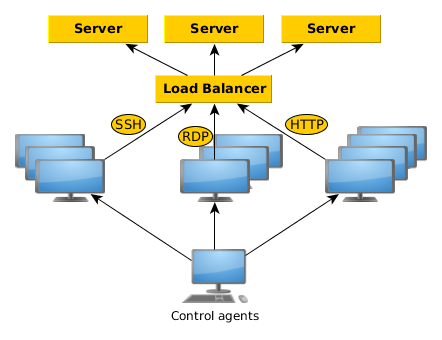
\includegraphics[width=13cm,keepaspectratio]{generator.png}
          \caption{Teljes rendszer}
      \label{fig:generator}
\end{figure}

\newpage
%\renewcommand{\bibname}{Irodalomjegyzék}
%\bibliographystyle{pemik}
%\bibliography{irodalomjegyzek}

\begin{thebibliography}{99}

     \bibitem{website:balabit}
        https://www.balabit.com/hu 
        (letöltés dátuma 2015. december 8.)\\
        {\em BalaBit IT Biztonságtechnikai Kft. \\}     

     \bibitem{website:zorp}
        https://www.balabit.com/hu/network-security/zorp-gpl
        (letöltés dátuma 2015. december 8.)\\
        {\em Zorp GPL tűzfal \\}     

    \bibitem{article:zorparticle}
		http://www.linuxjournal.com/article/7296
        {\em Mar 01, 2004  By Mick Bauer \\}     
        Paranoid Penguin - Application Proxying with Zorp, Part I 
        
     \bibitem{website:ubuntuzorp}
        http://packages.ubuntu.com/precise/net/zorp
        (letöltés dátuma 2015. december 8.)\\
        {\em Ubuntu Zorp csomag \\}    
    
    \bibitem{website:sso}
        https://en.wikipedia.org/wiki/Single\_sign-on
        (letöltés dátuma 2015. december 8. \\
        {\em SSO autentikáció \\}
           
     \bibitem{website:tcpdump}
        http://www.tcpdump.org/
        (letöltés dátuma 2015. december 8. \\
        {\em TCPDUMP főoldala\\}     
        
     \bibitem{website:wireshark}
         https://www.wireshark.org/
         (letöltés dátuma 2015. december 8.)\\
        {\em Wireshark hálózati analizáló program \\}         
        
     \bibitem{website:iperf}
        https://iperf.fr/
        (letöltés dátuma 2015. december 8.)\\
        {\em Iperf hálózattesztelő eszköz \\}
       
                       
     \bibitem{website:git}
		https://github.com/
		(letöltés dátuma 2015. december 8.)\\
        {\em GitHub verziókövető rendszer\\}
        
                        
     \bibitem{website:gummi}
		https://en.wikipedia.org/wiki/Gummi\_\%28software\%29
		(letöltés dátuma 2015. december 8.)\\
        {\em Gummi Latex szerkesztő program \\}
        
         
     \bibitem{website:yed}
		https://www.yworks.com/products/yed
		(letöltés dátuma 2015. december 8.)\\
        {\em yEd diagram szerkesztő\\}
       
     \bibitem{website:qt}
        http://www.qt.io/about-us/
        (letöltés dátuma 2015. december 8.)\\
        {\em Qt - About Us \\}
                

     \bibitem{website:vbox}
        https://www.virtualbox.org/
        (letöltés dátuma 2015. december 8.)\\
        {\em VirtualBox virtuális gép kezelő \\}
        
     \bibitem{website:linuxmint}
        http://www.linuxmint.com/release.php?id=22
        (letöltés dátuma 2015. december 8.)\\
        {\em Linux Mint 17 operációs rendszer\\}
        
    \bibitem{book:python}
		Cody Jackson (2013). \\
        {\em Learning to Program Using Python \\}
        

    \bibitem{website:end2end}
        http://www.tutorialspoint.com/software\_testing\_dictionary/end\_to\_end\_testing.htm
        (letöltés dátuma 2015. december 8.)\\
    {\em end-to-end teszt leírás \\}

    \bibitem{website:protobuf}
        https://developers.google.com/protocol-buffers/
        (letöltés dátuma 2015. december 8.)\\
    {\em Google Protocol Buffer fejlesztői dokumentáció\\}


\end{thebibliography}


\section{Mellékletek}

\subsection{CD melléklet}
A szakdolgozat CD mellékletének könyvtárszerkezete:

% itt a csel a [], amivel nem rak ki pontokat a latex
\begin{itemize}
    \item[] /KranitzGabor-TZ906Y-szakdolgozat.pdf
    \item[] /szakdolgozat-forraskod
    \begin{itemize}
        \item[] /kepek\_diagramok
        \item[] /szakdolgozat.tex
    \end{itemize}
    
    \item[] /virtualis\_gep
    \item[] /internetes\_hivatkozasok

\end{itemize}

\begin{figure}[h]
  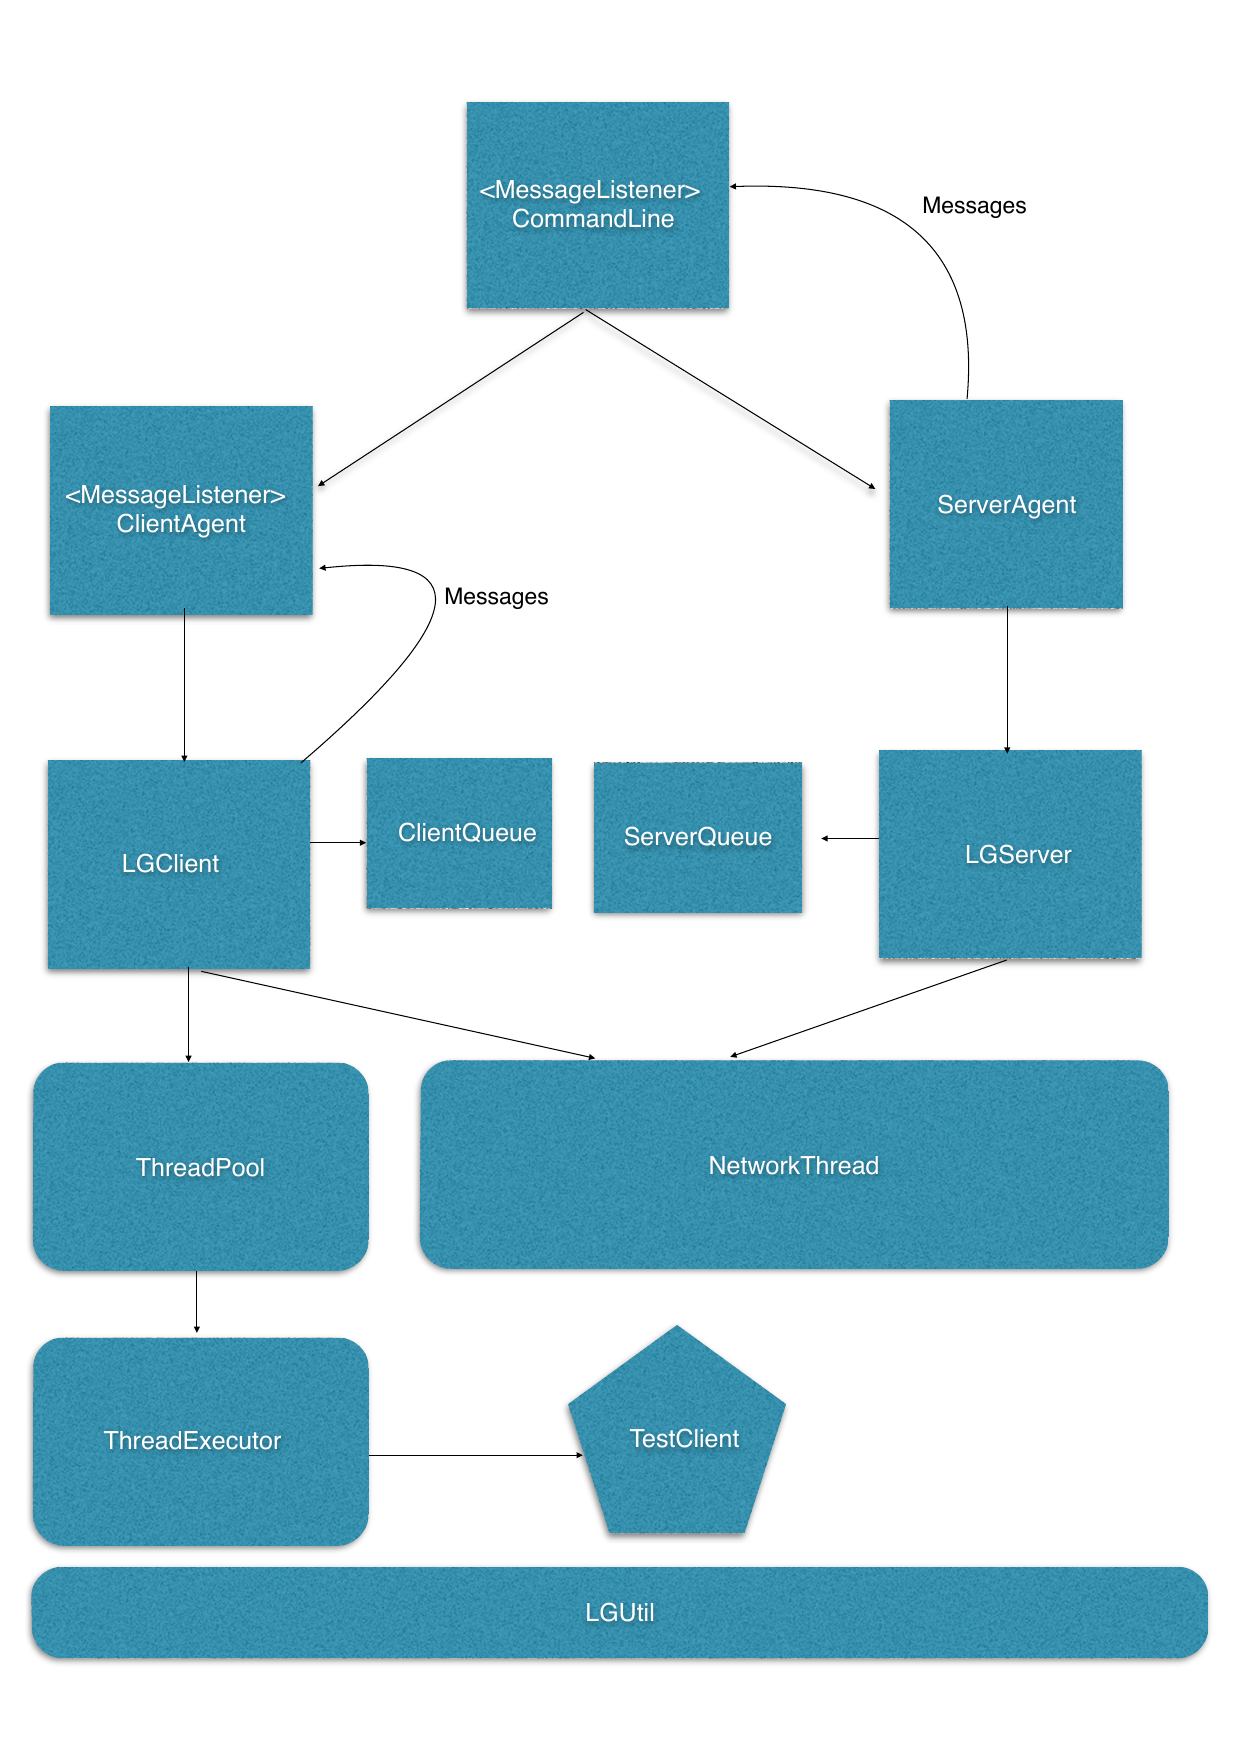
\includegraphics[width=1\textwidth]{load_generator.png}
  \caption{A keretrendszer felépítése }
  \label{fig:load_generator}
\end{figure}

\end{document}